\documentclass[11pt]{article}
\usepackage[margin=1in]{geometry}
\usepackage[T1]{fontenc}
\usepackage[sc]{mathpazo}
\linespread{1.08}
\usepackage{microtype}
\usepackage{amsmath,amssymb}
\usepackage{graphicx}
\usepackage{booktabs,array}
\usepackage[round]{natbib}
\usepackage[font=small,labelfont=bf,labelsep=period,justification=justified]{caption}
\usepackage{placeins}
\usepackage{float}
\usepackage{fancyhdr}
\usepackage{titlesec}
\usepackage{xcolor}
\usepackage[colorlinks=true,linkcolor=navy,citecolor=navy,urlcolor=navy]{hyperref}
\definecolor{navy}{RGB}{0,51,102}
\renewcommand{\arraystretch}{1.12}
\graphicspath{{figures/}}
\newcommand{\bn}{\textrm{bn}}
\newcommand{\bp}{\textrm{bp}}

% section headings
\titleformat{\section}{\large\bfseries}{\thesection.}{0.6em}{}
\titleformat{\subsection}{\normalsize\bfseries}{\thesubsection}{0.6em}{}
\titlespacing*{\section}{0pt}{1.6em}{0.7em}
\titlespacing*{\subsection}{0pt}{1.2em}{0.5em}

% running head
\pagestyle{fancy}
\fancyhf{}
\fancyhead[L]{\small\itshape Chongmankhong --- When Stablecoins Run}
\fancyhead[R]{\small\thepage}
\renewcommand{\headrulewidth}{0.3pt}
\fancypagestyle{plain}{\fancyhf{}\fancyfoot[C]{\small\thepage}\renewcommand{\headrulewidth}{0pt}}

\title{\LARGE\bfseries When Stablecoins Run:\\[0.15em] Fire-Sale Spillovers to the Treasury Bill Market\\[0.6em]
\large\mdseries An Agent-Based Stress Test}
\author{\large Thanatchon Chongmankhong\thanks{Preliminary working paper, November 2026. Comments welcome.
Replication code, configuration and every table in this paper are reproducible from the accompanying
\texttt{stablerun} repository. Institutional figures used for calibration and the references cited here were
compiled without access to primary sources and are listed in the repository for verification; they should be
checked before this paper is cited. The model is a stress-testing tool, not a forecast.}}
\date{\normalsize November 2026}

\begin{document}
\maketitle
\thispagestyle{plain}

\begin{center}
\begin{minipage}{0.9\textwidth}
\small
\begin{center}\textbf{Abstract}\end{center}
\noindent Payment stablecoins have become large holders of US Treasury bills, and the GENIUS Act of 2025 will push
their reserves further into bills of 93 days or less. We build an agent-based stress test in which heterogeneous
holders exit on private signals, a visible depeg and peer behaviour; only authorised redeemers reach the issuer at
par, while everyone else sells on a secondary market where capital-constrained arbitrageurs convert discounts into
redemptions; the issuer pays through a liquidation waterfall and the bill market absorbs outright sales and
withdrawn auction demand with permanent and temporary price impact. Calibrated to the USDC episode of March 2023
and the USDT episode of May 2022, the model yields three results. First, at today's size a run on the largest
issuer moves three-month bill yields by roughly 20\,bp and sells essentially no bills outright: redemptions are
throttled by processing capacity and funded by run-off, so the externality takes the form of demand withdrawn at
auction rather than a fire sale, and the issuer's own fire-sale losses are negligible because bill duration is
tiny. Second, scaling the sector, the 25\,bp mark is crossed at roughly 1.4--2 times today's size and the 50\,bp
mark at 5.5--8 times under square-root price impact; under linear impact (an upper bound) both are crossed
already today. Third, a cash buffer of 20--30\% of reserves removes the bill-market footprint of a liquidity run
and cuts that of a solvency run by two thirds; maturity caps convert outright sales into non-rollover; redemption
fees are ineffective; redeeming at net asset value rather than par halves the depeg. The single most important
unknown is how much redeemed cash returns to bills through money market funds.

\medskip
\noindent\textbf{Keywords:} stablecoins; Treasury bills; bank runs; fire sales; agent-based models; financial stability.\\
\textbf{JEL codes:} G01, G21, G23, E58.
\end{minipage}
\end{center}
\vspace{0.5em}

\section{Introduction}

Payment stablecoins are money-like liabilities backed by portfolios that look increasingly like those of
government money market funds. The two largest issuers alone report well over \$200\,bn of US Treasury bills,
reverse repo and government money market fund shares, and the GENIUS Act signed in July 2025 confines permitted
reserve assets to cash, insured deposits, bills with no more than 93 days to maturity, Treasury-backed repo and
government money market funds \citep[][all institutional figures used in this paper are listed for verification in
the repository]{genius2025}. A growing empirical literature documents that stablecoin flows already move the front
end of the Treasury curve in normal times \citep{ahmed2025}, and the Treasury Borrowing Advisory Committee has
discussed stablecoins as a structural source of bill demand \citep{tbac2025}.

What happens to that demand when a stablecoin runs? Two episodes give partial answers. In May 2022 Tether redeemed
roughly a tenth of its supply in two weeks after the collapse of Terra, with a brief and shallow depeg. In March
2023 USDC fell to about 88 cents over a weekend after Circle disclosed that \$3.3\,bn of its reserves sat at
Silicon Valley Bank, recovered within two days once deposits were guaranteed, and still lost about a quarter of
its supply over the following month \citep{circle2023,tether2022}. Neither episode disturbed the bill market, but
neither involved an issuer of today's size, let alone the multiples that industry projections contemplate. The
question this paper asks is quantitative: when a run happens, how much bill-market dislocation does the forced
liquidation of reserves cause, through which channel, and at what sector size does it become a financial-stability
concern?

Two episodes are too few for econometrics, so we answer with a calibrated agent-based model. Holders are
heterogeneous in size, information, attention and access to the issuer: institutions and arbitrageurs can redeem
at par, retail and most exchanges can only sell on a secondary market. Exit decisions follow a global-games-style
threshold rule on a private signal about reserve impairment, a visible depeg, peer behaviour and a suspension
flag. The secondary price carries a fundamental discount (the expected loss share of whoever remains) and a
liquidity discount proportional to the stock of tokens that arbitrageurs have not yet absorbed. The issuer pays
redemptions through a waterfall (cash, repo, money market fund shares, bills shortest-first, other assets at a
haircut), subject to a daily processing capacity, and manages liquidity by keeping cash for pending claims and
rolling the rest of its maturing bills. The bill market absorbs outright sales and demand withdrawn at auction
with a persistent and a temporary impact component, a dealer-capacity penalty and a reinvestment leak through
which redeemed cash returns via money market funds. A second issuer receives a belief spillover from the first.
The model nests a closed-form threshold aggregate when the behavioural channels are switched off, and we show
that the simulation reproduces it exactly.

Our contribution is threefold. First, we quantify the spillover and identify its channel. At today's size a run on
the largest issuer, whether a liquidity scare or a 10\% loss of reserves, moves three-month bill yields by
17--21\,bp in the model, and the issuer sells no bills outright: with processing capacity of about 1.2\% of
supply per day, redemptions are funded entirely by the \$2.8\,bn a day of maturing bills. The externality is
demand withdrawn at auction, not a fire sale, and the issuer's fire-sale loss is negligible because the bills it
would sell have a duration of weeks. Second, we turn ``stablecoins might be systemic one day'' into a number. Under
square-root impact, the 25\,bp threshold is crossed at 1.4--2 times today's size and the 50\,bp threshold at
5.5--8 times; under linear impact, the upper bound, both are crossed already today. Third, we rank levers. A
minimum cash buffer of 20--30\% removes the footprint of a liquidity run and cuts that of a solvency run by about
two thirds; the 93-day maturity cap converts outright sales into orderly non-rollover; redemption fees do
little; redeeming at net asset value rather than par halves the depeg; a Fed backstop that halves impact halves
the footprint by construction. Sensitivity analysis shows a clean separation: the size of a run is governed by
behavioural parameters (thresholds, attention, the perceived probability of loss), whereas its Treasury-market
footprint is governed by plumbing (how much redeemed cash returns to bills, arbitrage capital, the accounting of
non-rollover) and barely by behaviour at all.

The rest of the paper proceeds as follows. Section~\ref{sec:background} sets out the institutional mechanics.
Section~\ref{sec:lit} relates the paper to the literature. Section~\ref{sec:model} presents the model,
Section~\ref{sec:calib} its calibration and validation, Section~\ref{sec:results} the results,
Section~\ref{sec:robust} robustness, Section~\ref{sec:policy} policy implications. Section~\ref{sec:conclusion}
concludes. Appendices give the parameter table, pseudo-code and additional figures. Code, configuration and every
table in this paper are reproducible from the repository with one command.

\section{Institutional background}\label{sec:background}

\paragraph{Redemption mechanics.} A payment stablecoin is a token redeemable at par from its issuer, but direct
redemption is available only to verified counterparties above a minimum size: for the largest offshore issuer,
verified customers with a minimum of \$100,000 and a 0.1\% fee; for the largest US-regulated issuer, institutional
customers of its minting platform \citep{tether_attest,circle_reserve}. Everyone else obtains dollars by selling the
token on exchanges. The peg is therefore maintained by arbitrageurs who buy discounted tokens on the secondary
market and redeem them at par, and the depth of that arbitrage is bounded by their capital and by the issuer's
processing capacity \citep{ma2023,lyons2023}. During the USDC weekend of March 2023, redemption was unavailable
because banks were closed, arbitrage capital stood aside, and the secondary price cleared at a discount of about
twelve cents. Once redemption resumed and the Silicon Valley Bank exposure was resolved, the discount closed in a
day, but holders who had decided to leave kept redeeming through the following weeks.

\paragraph{Reserve rules.} The GENIUS Act requires one-for-one backing in US coins and currency, insured deposits,
Treasury bills with at most 93 days to maturity, Treasury-backed repo and reverse repo, shares of government money
market funds invested in the same assets, and central bank reserves; issuers must publish monthly reserve reports
and disclose their redemption policy, and may not pay interest to holders \citep{genius2025}. Issuer attestations at
mid-2026 report reserve mixes that already resemble this list: the largest offshore issuer holds roughly two thirds
of its assets in bills directly, with reverse repo, money market fund shares and a residual of other assets
(bitcoin, gold, secured loans); the largest US-regulated issuer holds about an eighth in bank deposits and the rest
in a government money market fund that invests in short bills and overnight repo \citep{tether_attest,circle_reserve}.
These are the two reserve profiles we model as ``Issuer~A'' and ``Issuer~B''; the figures are defaults from public
reports as remembered by the authors and must be replaced with the latest attestation before publication.

\paragraph{The bill market.} Treasury bills outstanding are of the order of \$6--7\,tn, with daily trading volume
in the hundreds of billions; money market funds and foreign official holders are the largest holders, and primary
dealers intermediate secondary trading subject to balance-sheet constraints that proved binding in March 2020
\citep{duffie2020,vissing2021,he2022}. Two features matter for a stablecoin run. First, bills are the most liquid
instrument in the world, so the price impact of even large flows is measured in basis points, not percent; the
empirical elasticity of three-month bill yields to stablecoin flows is a few basis points per \$3--4\,bn over ten
days, with outflows mattering more than inflows \citep{ahmed2025}. Second, a bill portfolio self-liquidates: a
\$120\,bn ladder of bills with an average maturity of one to two months returns about \$3\,bn of cash every
business day without any sale. An issuer facing redemptions can meet them by not rolling its maturities, which
withdraws demand at auction rather than adding supply in the secondary market. Both channels affect yields; only
the second is a fire sale in the usual sense, and only the second touches dealer balance sheets.

\paragraph{The March 2020 analogue.} Prime money market funds lost about 15\% of assets in two weeks in March
2020, sold commercial paper and bills into dislocated markets, and were backstopped by the Money Market Mutual Fund
Liquidity Facility after ten days \citep{li2021,fed_mmlf2020}. We use this episode to discipline the behaviour of
other bill holders and the design of the backstop lever.

\section{Related literature}\label{sec:lit}

The paper sits at the intersection of three literatures. The first studies stablecoin runs. \citet{gorton2023}
argue that privately issued stablecoins are the wildcat banknotes of our time; \citet{anadu2023} document that
stablecoin flows during 2022--23 resembled money market fund runs and flights to safety; \citet{ma2023} show that
the centralisation of arbitrage, which we model as a capital- and capacity-constrained arbitrage bid, trades off
peg stability against run risk; \citet{lyons2023} study what keeps the peg; \citet{davernas2022} and
\citet{bertsch2023} provide theoretical models of stablecoin fragility; \citet{liao2022} and \citet{barthelemy2023}
analyse the growth of stablecoins and their reserve holdings; \citet{bis2025} frame the policy debate around the
singleness, elasticity and integrity of money. The second literature concerns runs and fire sales more generally.
Our threshold rule is a reduced form of the global-games equilibrium of \citet{goldstein2005}, in the tradition of
\citet{diamond1983}, and our fire-sale cost follows \citet{morris2016}, \citet{shleifer2011} and
\citet{greenwood2015}; the stress-testing use of fire-sale externalities follows \citet{cont2017}. The third
literature concerns the Treasury market: the price-impact anchor comes from \citet{ahmed2025}, the market-structure
and March 2020 evidence from \citet{duffie2020}, \citet{vissing2021}, \citet{he2022} and \citet{fleming2003}, and the
decomposition of impact into permanent and temporary components from \citet{kyle1985} and \citet{almgren2001}, with
the square-root shape documented by \citet{bouchaud2018}. Methodologically we follow the agent-based tradition
advocated by \citet{farmer2009} and use one-at-a-time and global sensitivity designs \citep{saltelli2008,morris1991}.
What is new is the bridge: a calibrated model in which run dynamics, redemption plumbing and bill-market impact are
in one place, so that the size of the spillover, its channel and the leverage of policy can be computed rather than
asserted.

\section{Model}\label{sec:model}

Time is discrete in business days $t=1,\dots,T$ with $T=30$. All quantities are vectorised over Monte Carlo
paths. We describe one issuer; the second issuer (Section~\ref{sec:e4}) is identical with a belief spillover.

\subsection{Holders}

There are $N=10{,}000$ holders of five types $k$: retail, exchanges and market makers, DeFi protocols,
institutional treasuries and arbitrageurs, with shares of supply $(30, 30, 20, 15, 5)\%$ and holdings drawn
lognormally within type. Only institutional holders and arbitrageurs have direct access to the issuer. At the
start of the run the public learns that a share $x$ of reserves is \emph{exposed} (for example, deposits at a
failed bank). A share $r\in[0,1]$ of the exposure is actually lost; the market assigns probability $\psi$ that an
unresolved exposure becomes a loss, so the expected loss is $\ell_0 = x\,[r + (1-r)\psi]$ until a resolution day
$t_R$ on which the public learns the realised loss $xr$. Because the issuer pays at par, the loss falls on whoever
has not left: the expected loss share of a remaining holder is
\begin{equation}
b_t \;=\; \ell_t\, S_0 / S_{t-1},
\end{equation}
where $\ell_t$ is the public expected loss as a share of initial supply and $S_t$ is remaining supply. Holder $i$
observes $b_t$ with a private noise $\varepsilon_i\sim N(0,\sigma^2)$ fixed over the episode, $x_{it}=b_t+\varepsilon_i$,
and forms an exit signal
\begin{equation}
s_{it} \;=\; w_2 x_{it} + w_3 H_t + w_4 \mathbf{1}[\text{suspended}_{t-1}] + \nu_t + w_1 (1-p_{t-1}),
\label{eq:signal}
\end{equation}
where $H_t = \lambda_H H_{t-1} + (\text{exit flow}_t / S_0)$ is a decaying herding state, $\nu_t\sim N(0,\sigma_\nu^2)$
is a common daily sentiment shock and $p_{t-1}$ is yesterday's secondary price. Holder $i$ pays attention on a given
day with a type-specific probability $a_k$ and exits if $s_{it}$ exceeds a threshold $\theta_i\sim N(\bar\theta_k,
\tau_k^2)$. An exited holder re-enters, buying tokens back at the market price, if the \emph{core} signal (the first
four terms of~(\ref{eq:signal}), without the depeg term) has fallen below $\theta_i - h$: once fundamentals are fine,
a discount is a buying opportunity rather than a reason to stay away. Direct-access holders who exit join the
issuer's redemption queue at par; all others sell on the secondary market.

The threshold rule is a reduced form of a global game. In \citet{goldstein2005}, agents with private signals about a
fundamental coordinate on a unique cutoff; here the cutoffs are heterogeneous by type because redemption access,
holding size and costs differ, and we calibrate their level rather than derive it. Appendix~\ref{app:benchmark}
shows that with the herding, depeg and suspension channels switched off and $b_t$ held fixed, the share of supply that
exits converges exactly to the closed-form aggregate $\sum_k \omega_k \Phi\!\big((x-\bar\theta_k)/\sqrt{\sigma^2+\tau_k^2}\big)$,
so the simulation nests a transparent benchmark.

\subsection{Secondary market and arbitrage}

Tokens offered on day $t$ are new sales $V_t$ plus the \emph{overhang} $O_{t-1}$ of tokens held by uninformed dip
buyers who resell. Demand at par from re-entering holders is served first. Arbitrageurs then buy
\begin{equation}
B_t \;=\; \min\!\big(V_t + O_{t-1} - \text{re-entry}_t,\; \kappa S_0,\; \max(0,\, h_a c S_0 - Q_{t-1})\big)
\end{equation}
if the discount covers the redemption fee plus their cost, where $\kappa$ is daily arbitrage capital as a share of
supply, $c$ the issuer's daily processing capacity as a share of supply, $h_a$ the number of days of capacity within
which they require their claim to clear, and $Q$ the redemption queue; a suspended issuer removes the arbitrage bid
entirely. The remainder stays as overhang and sets the liquidity discount. The secondary price is
\begin{equation}
p_t \;=\; \max\Big(1 - \min(b_t, \bar d) - \big[\,c_a \mathbf{1}[\text{offered}>0] + \eta\, O_t/S_0 + \delta\,
\mathbf{1}[\text{suspended}_t]\big],\; p_{\min}\Big),
\end{equation}
a fundamental discount equal to the expected loss share of remaining holders plus an inventory-type liquidity
discount proportional to the stock of unabsorbed tokens. Arbitrage purchases join the redemption queue at par.

\subsection{Issuer}

Reserves are held in cash and deposits, overnight reverse repo, money market fund shares, bills of at most one
month ($\text{tb1}$), bills of one to three months ($\text{tb3}$) and other assets. Impairment removes the realised
loss from the least liquid assets first (other, then cash, then money market fund shares, then repo); bills are never
impaired. Each day a uniform ladder matures: $\text{tb1}$ runs off into cash over 21 business days and $\text{tb3}$
rolls into $\text{tb1}$ over 42. The issuer processes $\min(Q_t, cS_0)$ through a waterfall: cash, repo and money
market fund shares (no price impact), then bills shortest-first at the current price concession, then other assets
at a 30\% haircut; if the waterfall cannot raise the cash the issuer is \emph{suspended} for the day. Liquidity
management is explicit: the issuer keeps cash for the pending claims it can pay within $h_c=5$ days and rolls the
rest of the day's maturities back into bills, so the cash buffer is spent, not rebuilt, during a run. Maturities
kept as cash are bill demand \emph{withdrawn} at auction. Net asset value marks bills at the current concession.
A policy switch lets the issuer redeem at net asset value instead of par, in which case the loss is shared pro
rata and $b_t$ does not grow with redemptions.

\subsection{Bill market}

Let $C_t$ be cumulative net demand withdrawn from the bill market, $C_t = \max(0,\, C_{t-1} + \text{sold}_t +
\omega\,\text{withdrawn}_t - \text{buys}_t)$, where a share $\rho$ of each day's redemption payments returns to
bills through money market funds after a lag $L$ (buys), and $\omega$ weights non-rollover relative to a sale.
Dealer inventory $I_t = (1-\alpha) I_{t-1} + \text{sold}_t - \text{buys}_t$ builds only from outright sales and is
absorbed by other holders at rate $\alpha$. The three-month yield deviation from its no-run path is
\begin{equation}
Y_t \;=\; \underbrace{\lambda_P\, g(C_t)\, m_t}_{\text{persistent}} \;+\; \underbrace{(1-\kappa_T) Y^T_{t-1} +
\lambda_T\, g(\text{sold}_t)\, m_t}_{\text{temporary}}, \qquad m_t = 1 + (I_{t-1}/K)^{\gamma},
\label{eq:impact}
\end{equation}
with $g(q)=q$ for $q\le q_0$ and $g(q)=\sqrt{q_0 q}$ beyond the anchor flow $q_0=\$3.5\,\bn$ (square-root impact,
the baseline), or $g(q)=q$ throughout (linear impact, the upper bound). The coefficients are anchored so that a
\$3.5\,bn outflow raises the three-month yield by about 7\,bp after ten days, the outflow elasticity reported by
\citet{ahmed2025} (to be verified), with buys acting at a third of that strength. The fire-sale loss on bills sold is
face value times duration times the yield deviation, with durations of 0.04 and 0.17 years for the two buckets. A
Fed backstop, when active from day two, removes the dealer-capacity penalty and halves the impact coefficients, a
stylised Money Market Mutual Fund Liquidity Facility.

\subsection{Timing, outputs and experiments}

Within a day: beliefs and signals update; holders exit or re-enter; exits route to the queue or the secondary market;
the secondary market clears; the ladder runs off and the issuer processes the queue through the waterfall; the
issuer manages liquidity; the bill market updates; losses, net asset value and all series are recorded. Each
scenario is run for 1{,}000 Monte Carlo paths in the baseline and 200--300 in the grids; a path draws thresholds,
private signals and common shocks, and a run is defined as cumulative redemptions of at least 20\% of initial
supply by day 30. Five experiments follow the pre-registered design: E1 baseline shocks on Issuer~A, E2 scaling of
issuer size, E3 a policy grid, E4 contagion to Issuer~B, and E5 sensitivity.

\section{Calibration and validation}\label{sec:calib}

Table~\ref{tab:params} in Appendix~\ref{app:params} lists every parameter with its value and source. Issuer sizes
and reserve mixes are defaults from public attestations (\$180\,bn for Issuer~A with 66\% bills, 10\% reverse
repo, 4\% money market funds, 0.5\% cash and 19.5\% other assets; \$75\,bn for Issuer~B with 12\% deposits and
the rest in a government fund holding 40\% bills and 48\% repo on a look-through basis); both are flagged for
verification. Market-side parameters (impact coefficients, dealer capacity, reinvestment) are anchored on the
literature or set by assumption and varied in Section~\ref{sec:robust}.

The behavioural and plumbing parameters that the literature does not pin down are calibrated on two episodes. The
USDC episode of March 2023 is represented, for Issuer~B, as an 8\% exposure with no processing on business day~1
(the weekend) and resolution on day~2; targets are a trough of 0.87--0.88, redemptions of 12--15\% of supply in
the first week and about 25\% after a month. The USDT episode of May 2022 is represented, for Issuer~A, as a
feared exposure resolved after ten days of successful redemptions; targets are a trough of 0.95--0.97 and
redemptions of about 12\% in two weeks. All targets are from memory and listed for verification. A two-stage grid
fits the shared parameters (liquidity depth $\eta$, a common scale on the exit thresholds, the depeg weight $w_1$,
the loss probability $\psi$ and the size of the feared USDT exposure) jointly with issuer-specific processing
capacity and arbitrage capital, minimising the sum of squared standardised target errors. The best fit has
$\eta=0.1$, threshold scale~1, $w_1=0.5$, $\psi=1$, a feared USDT exposure of 2\%, processing capacity of 1.2\% of
supply per day for Issuer~A and 3\% for Issuer~B, and arbitrage capital of 1.1\% and 3\% of supply per day.

\begin{table}[tbp]\centering\small
\caption{Validation against the two calibration episodes (300 paths, 10{,}000 agents). $z$ is the model minus the
observed value in units of the tolerance. All observed values are to be verified.}\label{tab:validation}
\resizebox{\textwidth}{!}{\begin{tabular}{llrrr}
\toprule
Episode & Target & Observed (tol.) & Model & $z$ \\
\midrule
USDC, March 2023 (Issuer B) & Minimum price & 0.875 (0.010) & 0.904 & +2.9 \\
USDC, March 2023 (Issuer B) & Redeemed, 5 business days & 0.135 (0.015) & 0.120 & -1.0 \\
USDC, March 2023 (Issuer B) & Redeemed, 22 business days & 0.250 (0.030) & 0.240 & -0.3 \\
USDT, May 2022 (Issuer A) & Minimum price & 0.960 (0.015) & 0.925 & -2.3 \\
USDT, May 2022 (Issuer A) & Redeemed, 10 business days & 0.120 (0.015) & 0.120 & -0.0 \\
\bottomrule
\end{tabular}
}
\end{table}

\begin{figure}[tbp]\centering
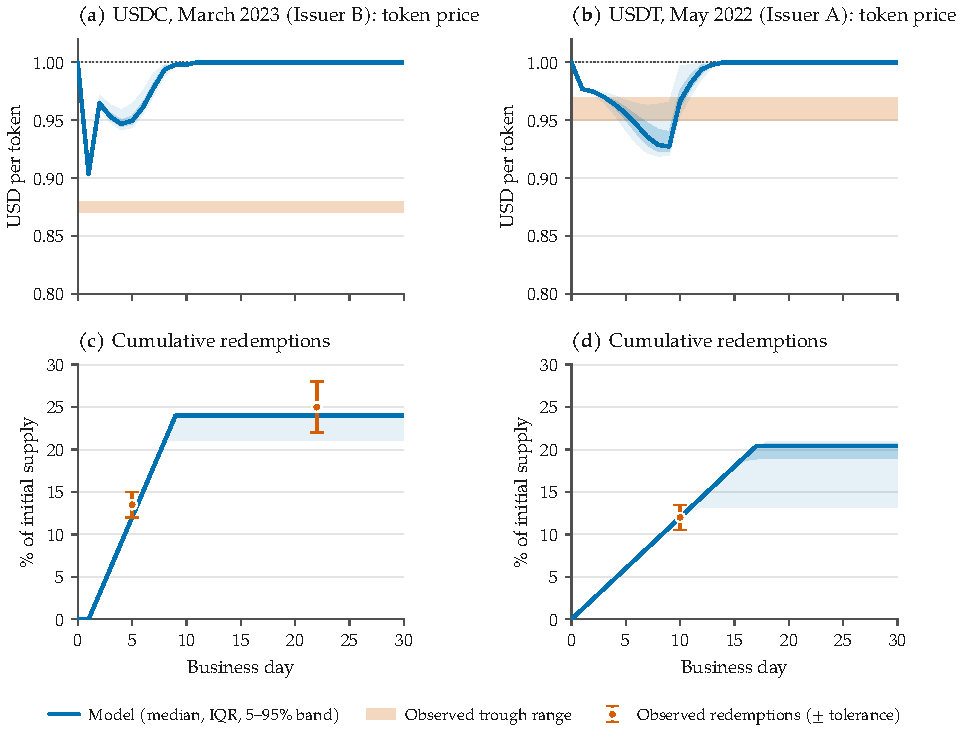
\includegraphics[width=\textwidth]{F4_validation}
\caption{Validation. Model paths (median, interquartile range and 5--95\% band) for the token price and cumulative
redemptions in the two calibration episodes, against the observed trough range and redemption targets (to be
verified).}\label{fig:f4}
\end{figure}

Table~\ref{tab:validation} and Figure~\ref{fig:f4} show the fit. Redemption volumes are matched in both episodes:
12\% of USDC supply in the first week against 12--15\% observed, 24\% after a month against 25\%, and 12\% of USDT
supply in two weeks. Processing capacity is the binding constraint in both, which is why the fitted capacities
are low: 1.2\% of supply per day is about \$2\,bn for Issuer~A, close to what Tether actually paid out per day in
May 2022, and 3\% is about \$2.3\,bn for Issuer~B. The model under-predicts the depth of the USDC trough (0.90
against 0.875) and over-predicts that of USDT (0.93 against 0.96); a single liquidity-depth parameter cannot
reproduce both a thin weekend crypto market with banks closed and a deep weekday market. We report this as a
limitation rather than add a weekend-specific parameter, and note that the discrepancy affects the price channel
only: the bill-market results below depend on redemption volumes and timing, which are matched.

\section{Results}\label{sec:results}

\subsection{Baseline dynamics (E1)}

\begin{figure}[tbp]\centering
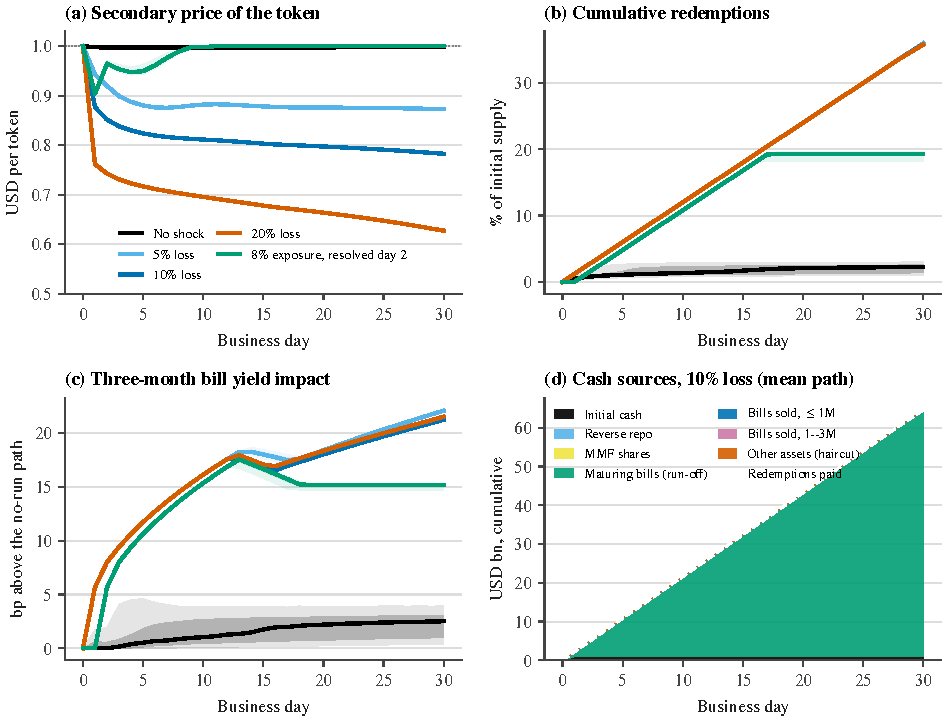
\includegraphics[width=\textwidth]{F1_A_baseline_dynamics}
\caption{Baseline run dynamics for Issuer~A (1{,}000 paths; lines are medians, bands the interquartile and 5--95\%
ranges). (a)~Secondary price; (b)~cumulative redemptions; (c)~three-month bill-yield impact; (d)~cash sources that
funded redemptions in the 10\% loss scenario (mean path): the dashed line is cumulative redemptions paid.}
\label{fig:f1}
\end{figure}

\begin{table}[tbp]\centering\small
\caption{E1 baseline, Issuer~A, 1{,}000 Monte Carlo paths, 30 business days. Medians across paths unless stated.
``Resolved'' = 8\% of reserves exposed, no processing on day~1, exposure resolved without loss on day~2.}
\label{tab:e1}
\resizebox{\textwidth}{!}{\begin{tabular}{@{}lrrrrr@{}}
\toprule
 & No shock & 5\% loss & 10\% loss & 20\% loss & \begin{tabular}[b]{@{}r@{}}8\% exposure,\\resolved day 2\end{tabular} \\
\midrule
\multicolumn{6}{@{}l}{\itshape Run} \\
\quad Minimum token price & 0.997 & 0.872 & 0.783 & 0.628 & 0.904 \\
\quad Redeemed by day 7 & 1.2\% & 8.4\% & 8.4\% & 8.4\% & 7.2\% \\
\quad Redeemed by day 30 & 2.2\% & 36.0\% & 35.8\% & 35.8\% & 19.3\% \\
\quad P(redemptions $\geq$ 20\%) & 0\% & 100\% & 100\% & 100\% & 0\% \\
\quad P(redemptions $\geq$ 50\%) & 0\% & 0\% & 0\% & 0\% & 0\% \\
\quad P(any suspension day) & 0\% & 0\% & 0\% & 0\% & 0\% \\
\addlinespace
\multicolumn{6}{@{}l}{\itshape Treasury-bill market} \\
\quad Peak three-month yield impact, bp & 4.2 & 22.1 & 21.2 & 21.5 & 17.5 \\
\quad Peak impact, bp, 95th percentile & 5.8 & 22.2 & 21.3 & 21.5 & 17.6 \\
\quad Bills sold outright, \$bn & 0.0 & 0.0 & 0.0 & 0.0 & 0.0 \\
\quad Maturing bills not rolled, \$bn & 3.1 & 66.1 & 63.5 & 64.3 & 33.9 \\
\quad Peak net bill demand withdrawn, \$bn & 2.1 & 34.8 & 32.2 & 33.1 & 22.0 \\
\addlinespace
\multicolumn{6}{@{}l}{\itshape Issuer} \\
\quad Other assets sold, \$bn & 0.0 & 0.0 & 0.0 & 0.0 & 0.0 \\
\quad Fire-sale and haircut loss, \$bn & 0.00 & 0.00 & 0.00 & 0.00 & 0.00 \\
\quad Net asset value on day 30 & 1.000 & 0.923 & 0.845 & 0.690 & 1.000 \\
\bottomrule
\end{tabular}
}
\end{table}

Figure~\ref{fig:f1} and Table~\ref{tab:e1} show Issuer~A under five shocks: no shock, a realised loss of 5, 10 or
20\% of reserves, and the calibrated liquidity scare. Three features stand out. First, a realised loss of any size
in this range produces a run: redemptions reach 8.4\% of supply in the first week and 36\% by day 30 in all three
loss scenarios, and the probability of a run is one. The run is not larger because it cannot be faster:
processing capacity binds for the first three weeks and arbitrage capital thereafter, so the loss scenarios
differ only in price, which settles at one minus the loss share of the remaining holders minus a liquidity
discount (0.87, 0.78 and 0.63 for the 5, 10 and 20\% losses) and keeps drifting down as the loss concentrates on
those who stay. Second, the liquidity scare looks different: the price falls to 0.90 while redemption is closed,
recovers fully within two weeks as re-entering holders absorb the overhang, and redemptions stop at 19\% of
supply, just below the run threshold. Third, and most important for the Treasury market, the issuer sells no bills
outright in any scenario. Panel~(d) shows why: with processing capacity of about \$2.2\,bn a day and \$2.8\,bn of bills
maturing every business day, every dollar of redemptions is paid out of run-off, and reverse repo and money market
fund shares are never touched. The issuer stops rolling those maturities while it has pending claims; over the month it withholds \$63\,bn of auction demand in the 10\% loss scenario, about half of
which returns through money market funds, for a peak net demand withdrawal of \$32\,bn and a peak three-month
yield impact of 21\,bp. The fire-sale loss is zero because nothing is sold, and even where bills are sold in
later experiments it stays below \$10\,m: a bill with six weeks to maturity sold 60\,bp cheap loses seven basis
points of face value. The externality falls on the Treasury market, not on the issuer.

Issuer~B behaves differently (Appendix~\ref{app:extra}, Table~\ref{tab:e1B}). Its reserves contain no cushion of
other assets to absorb an impairment, so a realised loss hits deposits and the fund directly; with faster
processing (3\% a day) it pays out 80--90\% of supply within the month in the loss scenarios, sells up to \$8\,bn
of bills once repo is exhausted, and suspends in the 10\% and 20\% loss scenarios when the remaining holders are
left with nothing. Its liquidity scare ends with 24\% of supply redeemed, the USDC outcome it was calibrated to.

\subsection{Tipping point (E2)}

\begin{figure}[tbp]\centering
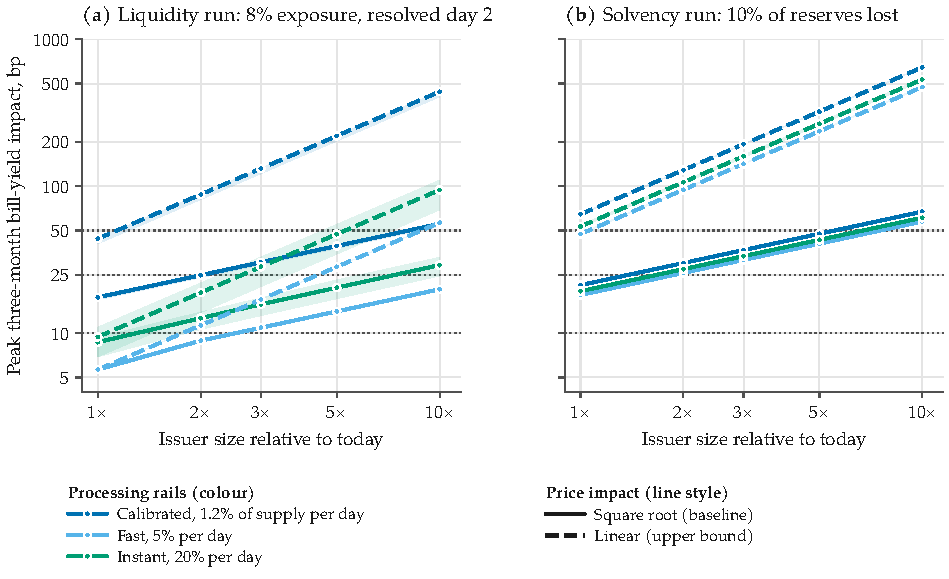
\includegraphics[width=\textwidth]{F2_tipping_point}
\caption{Peak three-month bill-yield impact against issuer size (log scales, medians with 5--95\% bands, 300
paths). ``Rails'' is daily processing capacity as a share of supply: calibrated (1.2\%), fast (5\%) or instant
(20\%). Dotted lines mark 10, 25 and 50\,bp.}\label{fig:f2}
\end{figure}

\begin{table}[tbp]\centering\small
\caption{E2: median peak three-month bill-yield impact (bp) by issuer size, and the size at which it first exceeds
10, 25 and 50\,bp (log-linear interpolation). Issuer~A, 300 paths per cell.}\label{tab:e2}
\resizebox{\textwidth}{!}{\begin{tabular}{@{}lllrrrrrrrr@{}}
\toprule
 &  &  & \multicolumn{5}{c}{\begin{tabular}[b]{@{}c@{}}Peak impact, bp,\\at issuer size\end{tabular}} & \multicolumn{3}{c@{}}{\begin{tabular}[b]{@{}c@{}}Size at which\\impact first exceeds\end{tabular}} \\
\cmidrule(lr){4-8}\cmidrule(l){9-11}
Scenario & Price impact & Rails & 1$\times$ & 2$\times$ & 3$\times$ & 5$\times$ & 10$\times$ & 10 bp & 25 bp & 50 bp \\
\midrule
Liquidity run & Square root & Calibrated & 18 & 25 & 30 & 39 & 55 & $<1\times$ & 2.0$\times$ & 8.1$\times$ \\
 &  & Fast & 6 & 9 & 11 & 14 & 20 & 2.5$\times$ & $>10\times$ & $>10\times$ \\
 &  & Instant & 9 & 13 & 16 & 20 & 29 & 1.3$\times$ & 7.4$\times$ & $>10\times$ \\
 & Linear & Calibrated & 44 & 88 & 132 & 220 & 440 & $<1\times$ & $<1\times$ & 1.1$\times$ \\
 &  & Fast & 6 & 11 & 17 & 28 & 57 & 1.8$\times$ & 4.4$\times$ & 8.8$\times$ \\
 &  & Instant & 9 & 19 & 28 & 47 & 94 & 1.1$\times$ & 2.6$\times$ & 5.3$\times$ \\
\addlinespace
Solvency run & Square root & Calibrated & 21 & 30 & 37 & 47 & 67 & $<1\times$ & 1.4$\times$ & 5.5$\times$ \\
 &  & Fast & 18 & 26 & 32 & 41 & 58 & $<1\times$ & 1.9$\times$ & 7.5$\times$ \\
 &  & Instant & 19 & 27 & 33 & 43 & 61 & $<1\times$ & 1.7$\times$ & 6.7$\times$ \\
 & Linear & Calibrated & 64 & 129 & 193 & 322 & 644 & $<1\times$ & $<1\times$ & $<1\times$ \\
 &  & Fast & 47 & 95 & 142 & 237 & 473 & $<1\times$ & $<1\times$ & 1.1$\times$ \\
 &  & Instant & 53 & 107 & 160 & 266 & 533 & $<1\times$ & $<1\times$ & $<1\times$ \\
\bottomrule
\end{tabular}
}
\end{table}

Figure~\ref{fig:f2} and Table~\ref{tab:e2} scale Issuer~A to 2, 3, 5 and 10 times its current size, holding the
bill market fixed and scaling everything on the issuer's side (processing capacity, arbitrage capital, the ladder)
with it, so that the exercise isolates the market's capacity to absorb. Under square-root impact the peak yield
effect grows with roughly the square root of size: a solvency run moves three-month yields by 21\,bp today, 30\,bp
at twice today's size, 47\,bp at five times and 67\,bp at ten times; the liquidity scare moves them by 18, 25, 39
and 55\,bp. The 25\,bp threshold is crossed at 1.4 times today's size for a solvency run and 2 times for a scare;
the 50\,bp threshold at 5.5 and 8 times. Under linear impact, the upper bound in which every billion withdrawn costs
the same two basis points, both thresholds are crossed already at today's size and a tenfold issuer would move the
front end by several hundred basis points, a dislocation that would certainly trigger intervention.

Redemption speed matters, but not in the direction one might expect. Faster rails (5\% or 20\% of supply per day)
produce \emph{more} redemptions (52\% of supply instead of 36\% in a solvency run) but a \emph{smaller} yield
impact at small sizes: when the issuer can pay quickly it pays from cash and repo, the redeemed cash reaches money
market funds within two days and comes back to the bill market, and the net demand withdrawn is small. Slow rails
keep the issuer in a weeks-long state of pending claims in which it hoards maturities, so the slow configuration
withholds \$34\,bn of auction demand in a scare against \$18\,bn with fast rails. Only with instant rails and at
five to ten times today's size does the issuer sell bills outright in volume (\$24--48\,bn in a scare, \$27\,bn in a
solvency run), and even then dealer inventory never approaches its capacity because money-market-fund reinvestment
buys what dealers would otherwise warehouse. The dealer-capacity channel, which dominated March 2020, is
inactive in this model unless the reinvestment leak is closed (Section~\ref{sec:robust}).

\subsection{Policy levers (E3)}

\begin{table}[tbp]\centering\small
\caption{E3 policy grid: main effects. Each row averages the outcome over the other levers (96 cells per
configuration, 200 paths per cell). The liquidity run is at today's size with calibrated rails; the solvency run is
a 10\% loss at five times today's size with fast rails. ``Redemption basis'' rows are single runs without other
policies.}\label{tab:e3}
\resizebox{\textwidth}{!}{\begin{tabular}{@{}lrrrrrrrr@{}}
\toprule
 & \multicolumn{4}{c}{Liquidity run, today's size, calibrated rails} & \multicolumn{4}{c@{}}{Solvency run, 5$\times$ today's size, fast rails} \\
\cmidrule(lr){2-5}\cmidrule(l){6-9}
 & \begin{tabular}[b]{@{}r@{}}Impact,\\bp\end{tabular} & \begin{tabular}[b]{@{}r@{}}Redeemed\\by day 30\end{tabular} & \begin{tabular}[b]{@{}r@{}}Minimum\\price\end{tabular} & \begin{tabular}[b]{@{}r@{}}Bills sold,\\\$bn\end{tabular} & \begin{tabular}[b]{@{}r@{}}Impact,\\bp\end{tabular} & \begin{tabular}[b]{@{}r@{}}Redeemed\\by day 30\end{tabular} & \begin{tabular}[b]{@{}r@{}}Minimum\\price\end{tabular} & \begin{tabular}[b]{@{}r@{}}Bills sold,\\\$bn\end{tabular} \\
\midrule
\multicolumn{9}{@{}l}{\itshape Minimum cash buffer, share of reserves} \\
\quad 0\% & 7.1 & 19.4\% & 0.904 & 0 & 41.3 & 51.9\% & 0.747 & 153 \\
\quad 10\% & 4.3 & 19.4\% & 0.904 & 0 & 35.2 & 51.9\% & 0.747 & 65 \\
\quad 20\% & 0.0 & 19.4\% & 0.904 & 0 & 25.5 & 51.9\% & 0.747 & 14 \\
\quad 30\% & 0.0 & 19.4\% & 0.904 & 0 & 14.8 & 51.9\% & 0.747 & 0 \\
\addlinespace
\multicolumn{9}{@{}l}{\itshape Redemption fee} \\
\quad 0\% & 2.9 & 19.4\% & 0.904 & 0 & 30.3 & 51.9\% & 0.747 & 63 \\
\quad 0.5\% & 2.9 & 19.4\% & 0.904 & 0 & 29.7 & 51.9\% & 0.747 & 60 \\
\quad 1\% & 2.9 & 19.4\% & 0.904 & 0 & 29.0 & 51.9\% & 0.747 & 57 \\
\quad 2\% & 2.8 & 19.4\% & 0.904 & 0 & 27.9 & 51.9\% & 0.747 & 52 \\
\addlinespace
\multicolumn{9}{@{}l}{\itshape Maturity cap} \\
\quad 93 days & 5.2 & 19.4\% & 0.904 & 0 & 29.2 & 51.9\% & 0.747 & 3 \\
\quad 180 days & 3.1 & 19.4\% & 0.904 & 0 & 28.3 & 51.9\% & 0.747 & 47 \\
\quad None & 0.3 & 19.4\% & 0.904 & 0 & 30.1 & 51.9\% & 0.747 & 125 \\
\addlinespace
\multicolumn{9}{@{}l}{\itshape Fed backstop} \\
\quad Off & 3.8 & 19.4\% & 0.904 & 0 & 39.2 & 51.9\% & 0.747 & 58 \\
\quad On & 1.9 & 19.4\% & 0.904 & 0 & 19.3 & 51.9\% & 0.747 & 58 \\
\addlinespace
\multicolumn{9}{@{}l}{\itshape Redemption basis (single runs, no other policy)} \\
\quad Par & 17.6 & 19.4\% & 0.904 & 0 & 40.7 & 51.9\% & 0.747 & 13 \\
\quad Net asset value & 17.6 & 19.4\% & 0.904 & 0 & 36.9 & 52.6\% & 0.831 & 0 \\
\bottomrule
\end{tabular}
}
\end{table}

\begin{figure}[tbp]\centering
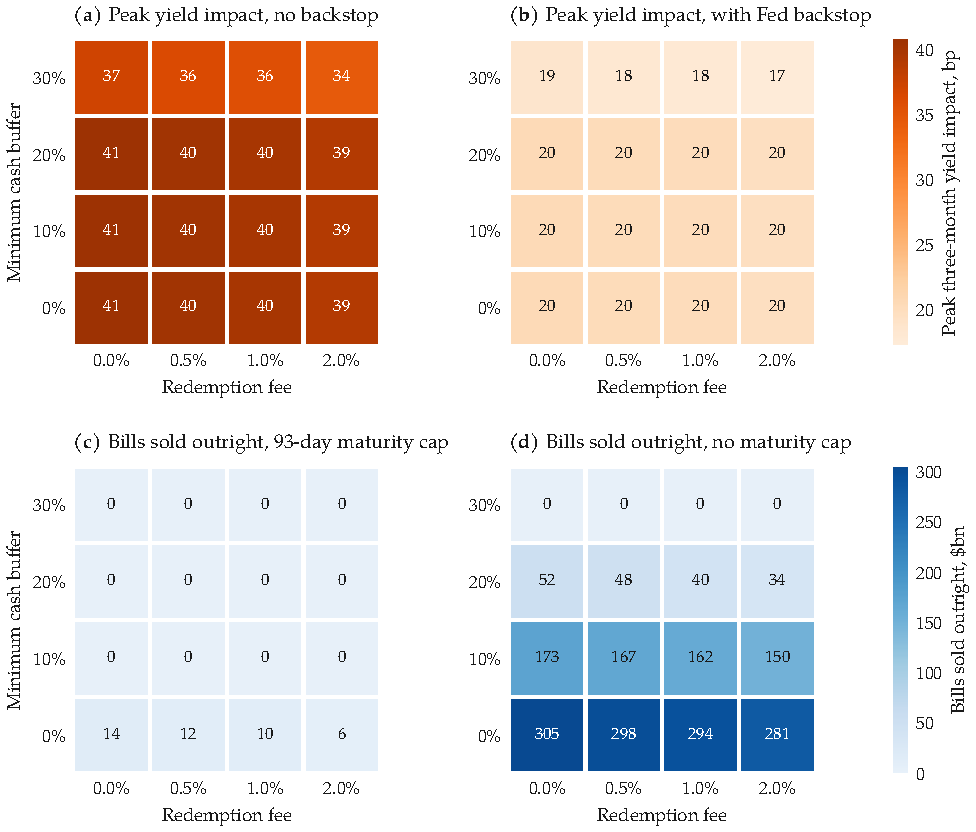
\includegraphics[width=0.92\textwidth]{F3_policy_heatmaps}
\caption{Policy grid for the solvency run at five times today's size with fast rails, by minimum cash buffer and
redemption fee. Top: peak bill-yield impact with the 93-day maturity cap, without and with a Fed backstop (shared
colour scale). Bottom: bills sold outright without a backstop, with the 93-day cap and with no cap.}\label{fig:f3}
\end{figure}

Table~\ref{tab:e3} and Figure~\ref{fig:f3} evaluate four levers on a full factorial grid, plus redemption at net
asset value, for a liquidity run at today's size and a solvency run at five times today's size with fast rails.
A \emph{minimum cash buffer} is the most powerful lever for the Treasury market: 20\% of reserves in cash removes
the bill-market footprint of the liquidity run entirely (from 7\,bp averaged over the grid to zero), and 30\% cuts
the solvency run's footprint from 41 to 15\,bp and the bills sold outright from \$153\,bn to zero, because the
buffer is spent before any bill is touched. It does nothing for the run itself: redemptions and the trough are
unchanged, since they are set by beliefs and processing. A \emph{maturity cap} trades one channel for the other:
with the 93-day cap the solvency run sells \$3\,bn of bills and withholds the rest through non-rollover, with a
180-day cap it sells \$47\,bn and with no cap \$125\,bn, while the measured yield impact barely changes because the
model prices withdrawn demand and outright sales alike. The cap therefore converts a dealer-balance-sheet event
into an auction-demand event, which is a gain in orderliness that the impact metric does not reward.
\emph{Redemption fees} of up to 2\% are ineffective: they shave two basis points off the impact and do not change
redemptions, because a holder facing a 10\% loss does not care about a 2\% fee and a scare resolves before the fee
binds. The \emph{Fed backstop} halves the footprint by construction (it halves the impact coefficients), so its
value in the model is the value of the assumption that a bill-purchase facility halves price impact; we include it
to show the scale of what a backstop must achieve rather than as a finding. Finally, \emph{redeeming at net asset
value} rather than par, the mutual-fund rule, does not stop the run (52.6\% against 51.9\% redeemed) but raises the
price trough from 0.75 to 0.83 and removes outright bill sales, because the loss no longer concentrates on those
who stay and the incentive to be first is weaker.

\subsection{Contagion (E4)}\label{sec:e4}

\begin{table}[tbp]\centering\small
\caption{E4 contagion: a shock to Issuer~A spills over to Issuer~B's beliefs with weight $\beta$ on A's depeg
(300 paths). ``Combined impact'' applies the persistent impact function to both issuers' net demand withdrawn.}
\label{tab:e4}
\resizebox{\textwidth}{!}{\begin{tabular}{@{}lrrrrrr@{}}
\toprule
 &  & \multicolumn{4}{c}{Issuer B} &  \\
\cmidrule(lr){3-6}
Shock to Issuer A & $\beta$ & \begin{tabular}[b]{@{}r@{}}Redeemed\\by day 7\end{tabular} & \begin{tabular}[b]{@{}r@{}}Redeemed\\by day 30\end{tabular} & \begin{tabular}[b]{@{}r@{}}Minimum\\price\end{tabular} & P(run) & \begin{tabular}[b]{@{}r@{}}Combined\\impact, bp\end{tabular} \\
\midrule
Liquidity run & 0.0 & 2.0\% & 2.3\% & 0.998 & 0\% & 17.5 \\
 & 0.3 & 14.0\% & 14.0\% & 0.967 & 9\% & 17.5 \\
 & 0.6 & 21.0\% & 30.0\% & 0.908 & 100\% & 17.5 \\
\addlinespace
Solvency run & 0.0 & 2.0\% & 2.3\% & 0.998 & 0\% & 21.2 \\
 & 0.3 & 21.0\% & 70.1\% & 0.879 & 100\% & 21.3 \\
 & 0.6 & 21.0\% & 90.0\% & 0.819 & 100\% & 21.2 \\
\bottomrule
\end{tabular}
}
\end{table}

Table~\ref{tab:e4} shocks Issuer~A and lets Issuer~B's holders add $\beta$ times A's depeg to their expected
loss. With $\beta=0.3$, a liquidity scare at A pulls 14\% of B's supply out at a trough of 0.97 and a solvency
run at A pulls 70\% out at 0.88; with $\beta=0.6$ B runs in every path. Yet the combined bill-market impact is
indistinguishable from A's alone, because B funds redemptions from deposits and repo and withdraws essentially no
bill demand. Contagion in this model is a peg and liquidity problem for the second issuer, not an additional
Treasury-market problem, as long as the second issuer's reserves are as liquid as Issuer~B's.

\section{Robustness}\label{sec:robust}

\begin{figure}[tbp]\centering
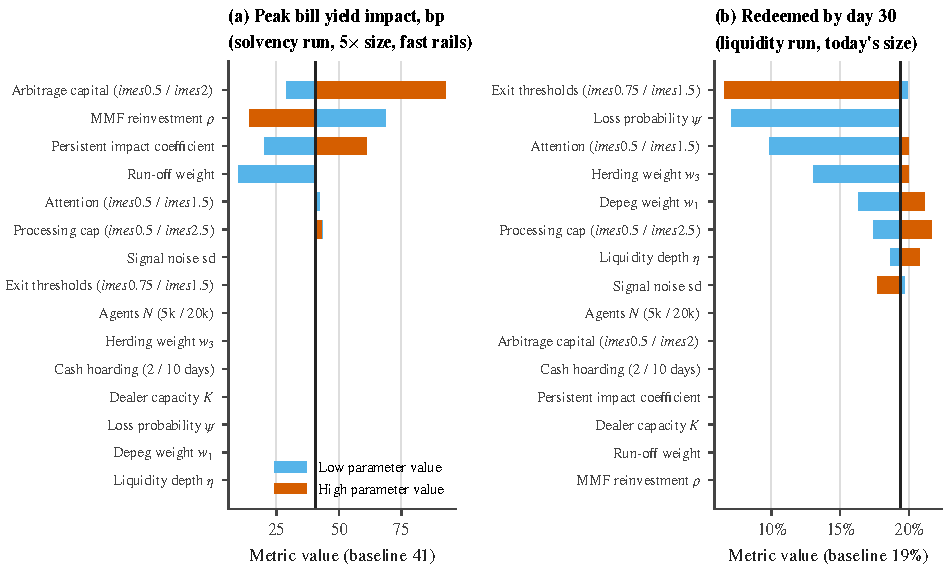
\includegraphics[width=\textwidth]{F5_sensitivity_tornado}
\caption{One-at-a-time sensitivity (200 paths). Bars show the change in the headline metric when each parameter is
moved to a low or high value, holding the others at baseline. (a)~Peak bill-yield impact in the solvency run at five
times today's size with fast rails; (b)~day-30 redemptions in the liquidity run at today's size.}\label{fig:f5}
\end{figure}

Figure~\ref{fig:f5} moves fifteen parameters one at a time between a low and a high value. The two panels tell
complementary stories. The Treasury-market footprint of a solvency run (panel~a) is governed by plumbing: the share
of redeemed cash that returns to bills through money market funds moves the peak impact between 14\,bp
($\rho=1$) and 69\,bp ($\rho=0$); the weight of non-rollover relative to a sale moves it between 10 and 41\,bp;
the persistent impact coefficient between 20 and 61\,bp; and arbitrage capital, which sets how fast the run can
proceed, between 29 and 93\,bp. The behavioural parameters (liquidity depth, thresholds, depeg and herding weights,
signal noise, attention) and dealer capacity move it by less than two basis points, and the number of agents by
none. The size of a liquidity run (panel~b) is the mirror image: day-30 redemptions range from 7\% to 20\% with
the threshold scale, from 10\% to 20\% with attention, from 7\% to 19\% with the loss probability $\psi$ and from
13\% to 20\% with herding, while every market-side parameter leaves them unchanged. The model's two halves are
separable, which is also why the imperfect fit of the price trough in Section~\ref{sec:calib} does not propagate
to the bill-market results.

Two further checks are in the appendices. Appendix~\ref{app:benchmark} shows that with the behavioural channels
off the simulation reproduces the closed-form threshold aggregate to within a tenth of a percentage point at every
loss share, so the heterogeneous-threshold machinery adds dynamics without distorting the static limit. The
linear-impact rows of Table~\ref{tab:e2} bound the results from above. Two robustness exercises in the
pre-registered design were not run: an hourly time step for the first five days, and a global (Sobol or Morris)
sensitivity design; the one-at-a-time design above is the first-order substitute and the hourly dynamics of the
USDC weekend are, as the validation showed, the part of the data the model fits least well.

\section{Policy implications}\label{sec:policy}

Five implications follow, each conditional on the model and on the verification of its inputs.

\emph{The channel is auction demand, not fire sales, at today's size.} An issuer with a self-liquidating bill ladder
and a processing throttle meets a run by not rolling maturities. The Treasury does not face a dealer dumping bills;
it faces a large buyer absent from the next several auctions. Monitoring should focus on issuers' rollover behaviour
and auction participation rather than on secondary-market sales, and the GENIUS Act's monthly reserve reports
should include ladder structure.

\emph{Size is the problem, and the threshold is not far.} Under the conservative square-root assumption, a run on an
issuer at one and a half to two times today's size moves three-month yields by 25\,bp, and at five to eight times by
50\,bp; under linear impact those marks are crossed today. The projections of a multi-trillion sector would, in this
model, put a stablecoin run in the same class as the March 2020 money market fund episode.

\emph{Cash buffers protect the Treasury market, not the peg.} A 20--30\% minimum cash share removes the footprint of
a liquidity run and most of a solvency run's, but changes nothing about how much is redeemed or how far the price
falls. Regulators who want to protect the bill market should mandate the buffer; those who want to protect holders
need the other levers.

\emph{Net-asset-value redemption weakens the stampede.} Paying at net asset value rather than par is the one lever
that improves the holder-side outcome, halving the depeg in a solvency run, because it removes the advantage of
being first. Redemption fees do not.

\emph{The reinvestment circuit is the key unknown.} Nothing in the model matters more for the Treasury market than
where redeemed cash goes. If it returns to bills through money market funds within days the system is a closed
circuit and the footprint is small; if it leaves for bank deposits or other assets the footprint quadruples and
dealer balance sheets come into play. This is an empirical question that the 2022 and 2023 episodes can answer and
that the model cannot.

\section{Conclusion}\label{sec:conclusion}

We built a calibrated agent-based stress test linking stablecoin run dynamics, redemption plumbing and Treasury-bill
price impact. At today's size a run on the largest issuer moves three-month bill yields by about 20\,bp through
withdrawn auction demand rather than fire sales, and the issuer's own fire-sale losses are negligible; the 25\,bp
mark is crossed at 1.4--2 times today's size and the 50\,bp mark at 5.5--8 times under square-root impact, and
already today under linear impact. Cash buffers and maturity caps shape the Treasury-market footprint, net-asset-value
redemption shapes the holder-side outcome, and fees shape neither. The model's two halves are separable: behaviour
sets the size of the run, plumbing sets its footprint.

The limitations are explicit. Reserve compositions and episode targets are from memory and must be verified;
the model fits redemption volumes well and price troughs less well; price impact is extrapolated from small
normal-times flows with a functional form that bounds rather than pins the answer; the dealer-capacity channel is
inactive unless reinvestment is slow; there are no inflows, no hourly dynamics and no bank-deposit channel; and the
model has two episodes of discipline. It is a stress-testing tool whose value lies in making the channels and the
orders of magnitude explicit, and in being reproducible: every number in this paper is regenerated from the
repository by one command.


\FloatBarrier
\bibliographystyle{plainnat}
\bibliography{refs}

\FloatBarrier
\appendix
\titleformat{\section}{\large\bfseries}{Appendix \thesection.}{0.6em}{}
\section{Parameter table}\label{app:params}

\begin{table}[H]\centering\footnotesize\renewcommand{\arraystretch}{1.0}\setlength{\tabcolsep}{4pt}
\caption{All model parameters (from \texttt{config/params\_default.yaml}, version 0.3). Where a row lists
several values they are in the order named in the parameter column. ``[verify]'' marks values taken from memory
of public sources that must be checked against the primary document.}\label{tab:params}
\adjustbox{max width=\textwidth}{\begin{tabular}{@{}>{\raggedright\arraybackslash}p{6.9cm}>{\raggedright\arraybackslash}p{4.6cm}>{\raggedright\arraybackslash}p{3.9cm}@{}}
\toprule
Parameter & Value & Source \\
\midrule
\multicolumn{3}{@{}l}{\itshape Issuers} \\
\hangindent=1em\hangafter=0 Supply, A / B, \$bn & 180 / 75 & attestations, 2026 [verify] \\
\hangindent=1em\hangafter=0 Reserves of A: cash / repo / MMF / bills $\leq$1M / bills 1--3M / other & 0.5\% / 10.0\% / 4.0\% / 33.0\% / 33.0\% / 19.5\% & attestation [verify] \\
\hangindent=1em\hangafter=0 Reserves of B: cash / repo / MMF / bills $\leq$1M / bills 1--3M / other & 12.0\% / 48.0\% / 0.0\% / 25.0\% / 15.0\% / 0.0\% & reserve report, look-through [verify] \\
\hangindent=1em\hangafter=0 Other-asset fire-sale haircut & 30\% & assumption \\
\hangindent=1em\hangafter=0 Bill ladder, tb1 / tb3, days & 21 / 42 & assumption \\
\hangindent=1em\hangafter=0 Processing capacity, A / B, \% of supply per day & 1.2\% / 3.0\% & calibrated \\
\hangindent=1em\hangafter=0 Arbitrage capital, A / B, \% of supply per day & 1.1\% / 3.0\% & calibrated \\
\hangindent=1em\hangafter=0 Redemption fee, A / B & 0.1\% / 0.0\% & issuer terms [verify] \\
\hangindent=1em\hangafter=0 Cash hoarding horizon, days & 5 & assumption \\
\addlinespace
\multicolumn{3}{@{}l}{\itshape Treasury-bill market} \\
\hangindent=1em\hangafter=0 Impact anchor flow, \$bn & 3.5 & Ahmed--Aldasoro [verify] \\
\hangindent=1em\hangafter=0 Persistent / temporary sell impact at the anchor, bp per \$bn & 2.0 / 1.0 & Ahmed--Aldasoro outflow range [verify] \\
\hangindent=1em\hangafter=0 Buy impact, bp per \$bn & 0.5 & asymmetry [verify] \\
\hangindent=1em\hangafter=0 Temporary impact decay per day & 0.3 & assumption \\
\hangindent=1em\hangafter=0 Impact shape & square root; linear below the anchor & square-root law \\
\hangindent=1em\hangafter=0 Dealer capacity $K$, \$bn / convexity $\gamma$ / absorption per day & 150 / 2.0 / 0.1 & assumption \\
\hangindent=1em\hangafter=0 MMF reinvestment share $\rho$ / lag, days & 0.5 / 2 & assumption \\
\hangindent=1em\hangafter=0 Duration of bills sold, tb1 / tb3, years & 0.04 / 0.17 & bucket midpoints \\
\addlinespace
\multicolumn{3}{@{}l}{\itshape Holders} \\
\hangindent=1em\hangafter=0 Agents $N$ & 10,000 & design \\
\hangindent=1em\hangafter=0 Type shares of supply: retail / exchange / DeFi / institutional / arbitrageur & 30\% / 30\% / 20\% / 15\% / 5\% & assumption \\
\hangindent=1em\hangafter=0 Attention probability per day, by type & 0.25 / 0.70 / 0.40 / 0.50 / 1.00 & assumption \\
\hangindent=1em\hangafter=0 Exit threshold mean, by type & 0.12 / 0.08 / 0.10 / 0.07 / 0.03 & calibrated (scale 1.0) \\
\hangindent=1em\hangafter=0 Exit threshold s.d., by type & 0.04 / 0.03 / 0.03 / 0.02 / 0.01 & assumption \\
\hangindent=1em\hangafter=0 Signal weights $w_1$, $w_2$, $w_3$, $w_4$ & 0.5, 1.0, 0.3, 0.2 & calibrated / assumption \\
\hangindent=1em\hangafter=0 Private-signal s.d. / common-shock s.d. & 0.02 / 0.005 & assumption \\
\hangindent=1em\hangafter=0 Herding memory / re-entry hysteresis & 0.6 / 0.02 & assumption \\
\hangindent=1em\hangafter=0 Loss probability $\psi$ & 1.0 & calibrated \\
\hangindent=1em\hangafter=0 Belief spillover $\beta$ (E4) & 0, 0.3, 0.6 & assumption \\
\addlinespace
\multicolumn{3}{@{}l}{\itshape Secondary market} \\
\hangindent=1em\hangafter=0 Liquidity depth $\eta$ / arbitrage cost / arbitrage horizon, days & 0.1 / 0.002 / 2 & calibrated / assumption \\
\hangindent=1em\hangafter=0 Suspension discount / price floor & 0.05 / 0.5 & assumption \\
\bottomrule
\end{tabular}
}
\end{table}

\section{Pseudo-code}\label{app:pseudo}

\begin{small}
\begin{enumerate}\setlength{\itemsep}{0pt}
\item Draw the population once per experiment: types, lognormal holdings within type, access flags, attention rates.
\item For each chunk of Monte Carlo paths: initialise reserves from the reserve shares; remove the realised loss from
  other assets, then cash, money market fund shares and repo; draw thresholds $\theta_i$ and private noise
  $\varepsilon_i$; set price $=1$, overhang, queue, herding state and dealer inventory to zero.
\item For each business day $t=1,\dots,30$:
  \begin{enumerate}\setlength{\itemsep}{0pt}
  \item Public expected loss $\ell_t$ (exposure times the loss probability until the resolution day, realised loss
    thereafter); belief $b_t=\ell_t S_0/S_{t-1}$ plus any spillover; signals $x_{it}=b_t+\varepsilon_i$; common
    shock $\nu_t$.
  \item Exit signal~(\ref{eq:signal}); agents who are awake and above threshold exit; exited agents whose core signal
    is below $\theta_i-h$ request re-entry.
  \item Route exits: direct-access holdings to the queue, others to secondary sales $V_t$; update $H_t$.
  \item Arbitrage capacity from daily capital, queue room within $h_a$ days of processing, suspension and the
    fee-plus-cost condition; serve re-entry demand, then arbitrage, from $V_t+O_{t-1}$; set the overhang and
    the price; accepted re-entrants rejoin the population pro rata.
  \item Queue $+=$ direct requests $+$ arbitrage purchases; ladder run-off ($\text{tb1}\to$ cash,
    $\text{tb3}\to\text{tb1}$); demand $=\min(Q_t, cS_0)$ (zero on blackout days); waterfall raises
    demand $\times$ payout (par or net asset value, net of fee); shortfall $\Rightarrow$ suspended; supply and queue fall
    by the tokens paid.
  \item Liquidity management: hoard $=\min(Q_t, h_c\, cS_0)$; reinvest $\min(\text{matured}, \max(0,\text{cash}-\text{hoard}))$
    into $\text{tb1}$; withdrawn $=$ matured $-$ reinvested.
  \item Bill market~(\ref{eq:impact}) with sold, withdrawn and the lagged reinvestment buys $\rho\cdot\text{paid}_{t-L}$;
    fire-sale loss; mark-to-market net asset value; record all series.
  \end{enumerate}
\item Metrics per path (minimum price, redemptions at days 7 and 30, peak impact, bills sold, demand withdrawn,
  suspension days, losses, net asset value) and summaries across paths (medians, 5th and 95th percentiles, run
  probabilities, threshold exceedance probabilities).
\end{enumerate}
\end{small}

\section{Analytic benchmark}\label{app:benchmark}

Consider a continuum of holders of type $k$ with supply shares $\omega_k$, a publicly known loss share $x$ of
reserves that does not change with redemptions, private signals $x_i = x+\varepsilon_i$ with $\varepsilon_i\sim
N(0,\sigma^2)$ and exit cutoffs $\theta_i\sim N(\bar\theta_k,\tau_k^2)$. In the limit without herding, depeg and
suspension channels, holder $i$ exits within the horizon if $x+\varepsilon_i>\theta_i$, so the share of supply that
exits is
\begin{equation}
E(x) \;=\; \sum_k \omega_k\, \Phi\!\left(\frac{x-\bar\theta_k}{\sqrt{\sigma^2+\tau_k^2}}\right).
\end{equation}
In a global game with a fire-sale liquidation cost $c(n)$ increasing in the exiting mass $n$, as in
\citet{goldstein2005} and \citet{morris2016}, the equilibrium cutoff $\theta^*$ falls as the liquidation cost
rises, $\partial\theta^*/\partial c<0$: a costlier fire sale makes the run start at a smaller loss. In our model the
fire-sale cost on bills is tiny because bill duration is tiny, so this amplification is absent and the cutoffs are
calibrated rather than derived. Table~\ref{tab:benchmark} and Figure~\ref{fig:f6} compare the simulated exit share
with $E(x)$ when $w_1=w_3=w_4=0$, $\sigma_\nu=0$ and the belief is held fixed: the two agree to within a tenth of a
percentage point.

\begin{table}[H]\centering\small
\caption{Benchmark check: share of supply exiting within 30 days in the simulation with the behavioural channels
off (100 paths) against the closed-form threshold aggregate.}
\label{tab:benchmark}
\begin{tabular}{rrr}
\toprule
Loss share & ABM exit share & Closed form \\
\midrule
0\% & 1.0\% & 1.1\% \\
2\% & 4.2\% & 4.3\% \\
4\% & 11.6\% & 11.6\% \\
6\% & 24.0\% & 24.0\% \\
8\% & 40.8\% & 40.9\% \\
10\% & 59.0\% & 59.0\% \\
12\% & 74.6\% & 74.6\% \\
15\% & 89.9\% & 90.0\% \\
20\% & 98.9\% & 98.8\% \\
\bottomrule
\end{tabular}

\end{table}

\begin{figure}[H]\centering
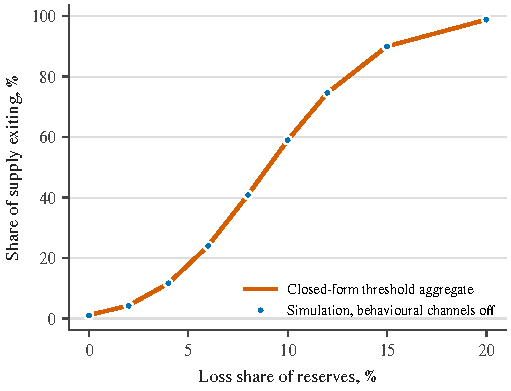
\includegraphics[width=0.55\textwidth]{F6_benchmark_check}
\caption{Benchmark check: simulated exit share with the behavioural channels off against the closed-form threshold
aggregate.}\label{fig:f6}
\end{figure}

\section{Additional results}\label{app:extra}

\begin{table}[H]\centering\small
\caption{E1 baseline for Issuer~B (1{,}000 paths). Same scenarios as Table~\ref{tab:e1}; Issuer~B has no cushion of
other assets, so a realised loss hits deposits and the reserve fund directly, and its processing capacity is 3\% of
supply per day.}\label{tab:e1B}
\adjustbox{max width=\textwidth}{\begin{tabular}{lrrrrr}
\toprule
Metric & No shock & 5\% loss & 10\% loss & 20\% loss & 8\% exposure, resolved \\
\midrule
Minimum token price (median) & 0.998 & 0.607 & 0.500 & 0.500 & 0.904 \\
Redeemed by day 7 & 1.9\% & 21.0\% & 21.0\% & 21.0\% & 18.0\% \\
Redeemed by day 30 & 2.3\% & 90.0\% & 90.0\% & 80.0\% & 24.0\% \\
P(redemptions $\geq$ 20\%) & 0\% & 100\% & 100\% & 100\% & 99\% \\
P(redemptions $\geq$ 50\%) & 0\% & 100\% & 100\% & 100\% & 0\% \\
Peak 3M bill-yield impact, bp (median) & 0.0 & 0.6 & 8.6 & 12.6 & 1.8 \\
Peak impact, bp (95th pct.) & 0.0 & 0.6 & 8.6 & 12.6 & 1.8 \\
Bills sold outright, \$bn & 0.0 & 0.4 & 4.3 & 7.7 & 0.0 \\
Maturing bills not rolled, \$bn & 0.0 & 25.9 & 25.7 & 22.3 & 7.1 \\
Peak net bill demand withdrawn, \$bn & 0.0 & 0.1 & 2.5 & 4.7 & 0.9 \\
Other assets sold, \$bn & 0.0 & 0.0 & 0.0 & 0.0 & 0.0 \\
P(any suspension day) & 0\% & 0\% & 100\% & 100\% & 0\% \\
Fire-sale and haircut loss, \$bn & 0.00 & 0.00 & 0.00 & 0.00 & 0.00 \\
NAV on day 30 (median) & 1.000 & 0.500 & 0.000 & 0.000 & 1.000 \\
\bottomrule
\end{tabular}
}
\end{table}

\begin{figure}[H]\centering
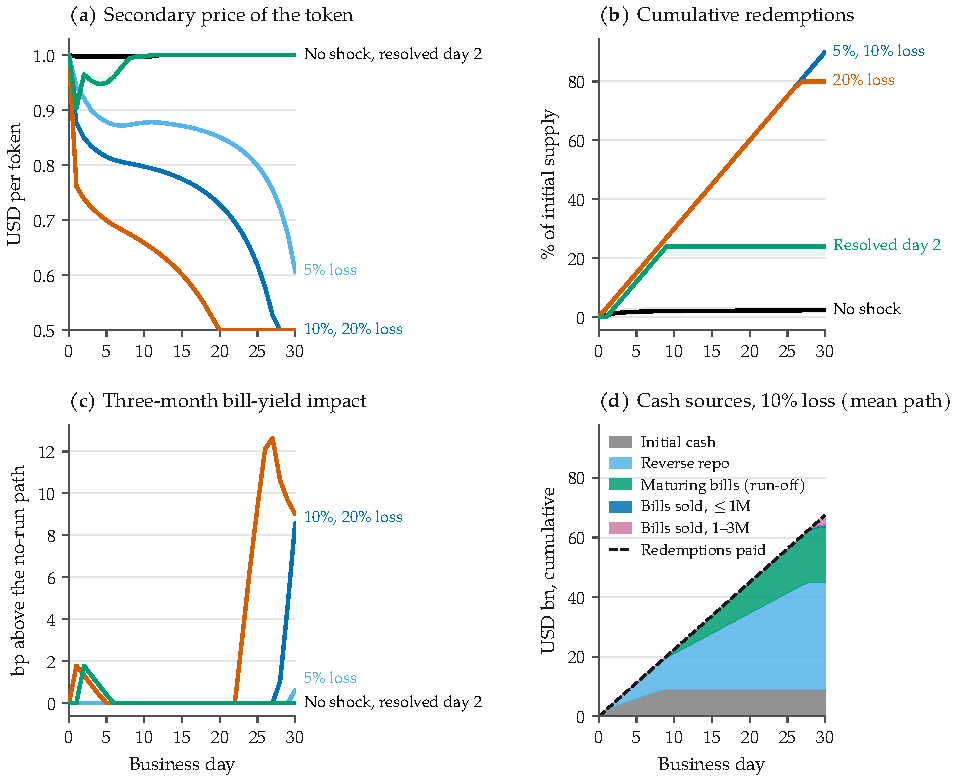
\includegraphics[width=\textwidth]{F1_B_baseline_dynamics}
\caption{Baseline run dynamics for Issuer~B (1{,}000 paths), panels as in Figure~\ref{fig:f1}.}\label{fig:f1b}
\end{figure}


\end{document}
